\documentclass[11pt]{article}

% ============================================================
% ARR SHORT PAPER SKELETON — IntentSpec
% Keep [review] for submission. Switch to \usepackage{acl}
% (no option) only for the camera-ready after acceptance.
% ============================================================
\usepackage[review]{acl}

\usepackage{times}
\usepackage{latexsym}
\usepackage[T1]{fontenc}
\usepackage[utf8]{inputenc}
\usepackage{microtype}    
\usepackage{inconsolata}   
\usepackage{graphicx}     

% 
\usepackage{booktabs}    
\usepackage{amsmath}    

\newcommand{\todo}[1]{\textcolor{red}{[TODO: #1]}}
\usepackage{xcolor} % needed for \todo above

\title{IntentSpec: How Much Does LLM-generated Code Violate Developer Intent?}

% Leave placeholder authors while [review] is on — the style file
% anonymizes the PDF, but keep real names out of the source you upload.
\author{First Author \\
  Affiliation \\
  \texttt{email@domain} \\\And
  Second Author \\
  Affiliation \\
  \texttt{email@domain} \\}

\begin{document}
\maketitle

% ============================================================
% ABSTRACT
% ============================================================
\begin{abstract}
Code generated by LLMs can violate a developer's implicit intentions when given an ambiguous prompt, yet standard benchmarks measure only whether code passes its stated tests. We introduce the Intent Violation Rate (IVR) and a 49-problem pilot benchmark derived from HumanEval+. Each problem strips implicit constraints from a clarified prompt and encodes them as hidden constraint tests. IVR measures the fraction of LLM-generated solutions that pass the stated (visible) tests yet fail hidden constraint tests that capture unstated intent. Evaluating Claude Sonnet 4.6, we find it passes 94.3\% of stated tests but violates intent in 54.5\% of problems, even when the code passes every stated test. These violations follow a systematic, bimodal pattern. Our findings indicate that pass rates overstate how well generated code reflects developer intent. 
\end{abstract}


% ============================================================
% 1. INTRODUCTION 
% ============================================================
\section{Introduction}

When LLMs are tasked with building code, they can understand the main task at hand, such as writing a function or script. However, these outputs are not always fully correct, requiring human-in-the-loop review and adjustments before they can be deployed. Developers, through review, will capture functional or logical errors, and cases where the code does something different from what they intended. Current benchmarks measure functional correctness of LLM generated code via a test pass rate \citep{austin2021program}, however, this metric does not capture whether the solution fully reflects what the developer intended. 

Test pass rates alone are insufficient as a metric because they do not detect intent violations, which refer to scenarios where LLMs will provide outputs that satisfy stated tests, but violate implicit constraints the developer assumes will be accounted for, and did not explicitly state. Prior work has documented similar failures in which LLMs produce code that will game specifications and exploit evaluation loopholes to pass tests without solving the intended task \citep{zhong2025impossiblebench}. We focus on a distinct failure mode: outputs that legitimately pass valid stated tests, but still violate unstated developer intent. To measure this, we propose the Intent Violation Rate (IVR), a metric that quantifies whether an output violates developer intent or not. We evaluate IVR on 49 algorithm specification problems, and demonstrate that Claude Sonnet 4.6 violates implicit developer constraints in approximately 54.5\% of cases, even when solutions pass stated tests. 


% ============================================================
% 2. RELATED WORK
% ============================================================
\section{Related Work}

When it comes to LLMs generating code, a big concern is when developers take the outputted code at face value due to a high pass rate on tests they built. Prior work defines code that passes provided test cases as having functional correctness \citep{austin2021program}, however \citet{chen2021codex} also note that models can pass weak test suites simply by deleting failing functionality. It has also been found that LLM generated code would often "overfit to assert statements", rather than properly apply logic \citep{austin2021program}. This meant LLMs would hardcode outputs for visible tests rather than actually create an accurate function that properly handled the general task at hand. A growing body of work also details LLMs that exploit evaluation shortcuts in code generation; this is seen in test suites where tasks were constructed to purposefully contradict specifications \citep{zhong2025impossiblebench}, or where outputs are hard coded, or tests were edited to pass \citep{gabor2025evilgenie}. Despite the focus on deliberate exploitation of flawed or gameable test suites, they further show that solutions passing held-out tests can still be incorrect. We build on this observation to measure violations of unstated intent in generated code that passes valid stated tests. 

By default, models rarely ask for clarification when a prompt is unclear, so when it comes to giving LLMs ambiguous prompts, prior work has seen a significant drop in test pass rates by approximately 80\% \citep{li2026clareval}. It shows that functional correctness (Pass@1) will fall apart when ambiguity is introduced to prompts, and we measure the intent violated in code where functional correctness holds. However, to address the drop in test pass rates, other work finds that by asking clarifying questions, the test pass rate of GPT-4's generated code saw an increase of approximately 10 points, rising from 70.96\% to 80.80\% in its functional correctness \citep{mu2023clarifygpt}. Additionally, \citet{kim2024aligning} finds that training models to recognize ambiguity and to ask, rather than guess, shows improvements in ambiguity detection. Rather than utilize methods to resolve ambiguity through interaction or prompt repair, IVR measures the intent violations that remain in code that passes its stated tests, generated from ambiguous prompts. 

% ============================================================
% 3. METHOD
% ============================================================
\section{Measuring Intent Violation Rate}

\subsection{Definition}
Intent Violation Rate, or IVR, is defined as follows: 
\begin{equation}
  \mathrm{IVR} = \frac{n_{\text{violating}}}{n_{\text{stated passed}}}
\end{equation}

Where for a given solution:
\begin{description}
  \item[$n_{\text{stated passed}}$:] number of generated solutions passing all stated tests
  \item[$n_{\text{violating}}$:] subset of those that fail $\geq 1$ hidden constraint test
\end{description}

IVR can be interpreted as: "Of the solutions that satisfy the given spec's visible tests, what fraction violates the developer's actual intent?" It is only measured over solutions that pass visible stated tests, therefore any solutions that do not pass the initial public test are not included in the calculation. The reported IVR is the mean of per-problem IVRs over problems that had $\geq 1$ solution passing stated test C1. 

\subsection{Benchmark Construction}
The built benchmark consists of 49 algorithm problems derived from HumanEval+ \citep{liu2023evalplus}. Each problem consists of an ambiguous prompt, a gold prompt, a stated test (C1), and hidden constraint tests (C2--C4, the number varying per problem). 

The selected HumanEval+ problems all contained a gold prompt, which we stripped down to produce an ambiguous prompt. In some cases, additional specifics were added to the gold prompt to further clarify the task at hand. This gold prompt was always hidden to the LLM, as it only received the ambiguous prompt, and C1, the stated test. Each aspect that was stripped from the gold prompt to formulate the ambiguous prompt was then used to create the hidden constraint tests. 

The scope was narrowed down to algorithm problems, where the prompt described a self contained function. A subset of these problems were cleanly decomposable into executable tests, and the formulation of the ambiguous prompt came from under specifying rather than misleading. Other task types, such as data transformation, involve fuzzier constraints and lack a comparable source at scale, being left to future work. 

As an example, the original HumanEval/34 prompt reads: \textit{"Return sorted unique elements in a list."}

We decompose it as shown in Table~\ref{tab:spec-example}: 
\begin{table}[ht]
\small
\centering
\begin{tabular}{@{}p{0.9cm}p{6cm}@{}}
\toprule
\multicolumn{2}{@{}l}{\textbf{HumanEval/34}} \\
\midrule
Ambig. & Return the unique elements in a list. \\
\addlinespace
Gold & Return only the unique values, sorted in
        ascending order. \\
\midrule
\textbf{C1} & \emph{stated}: only unique values \newline
  \texttt{solution([-2,4,4,6,6]) == [-2,4,6]} \\
\addlinespace
\textbf{C2} & \emph{hidden}: sorted ascending \newline
  \texttt{solution([-2,0,5,3,5,0,3])} \newline
  \texttt{== [-2,0,3,5]} \\
\bottomrule
\end{tabular}
\caption{Example spec pair. Stripping the sort-order
requirement from the gold prompt yields the ambiguous
prompt; C1 tests what remains stated, C2 tests the
stripped intent.}
\label{tab:spec-example}
\end{table}

To ensure the benchmark is sound, we applied two validation checks. First, a leakage audit was performed. When building the stated test, it must be satisfiable from the ambiguous prompt alone. During initial construction, 11 of the 49 problems failed this check. 9 of the failed tests were due to type errors, output format contamination, and hidden constraints leaking into the stated test. Of the hidden constraint leakage, what occurred was that the stated test also check a hidden constraint test, so a solution could not pass without already knowing part of the developer's intent. The other 2 problems were identified in the second validation check, where the canonical solution was run against the entire test suite to ensure stated and hidden tests were sound. These issues were errors in the tests themselves, something the initial leakage audit could not catch. Across all 49 problems, the validated references yield an IVR = 0, confirming that the hidden tests are satisfiable by correct code, and are not themselves the source of the measured violations. 

\subsection{Evaluation Pipeline}
The pipeline occurs in 4 stages: generation, execution, pass/fail determination, and IVR calculation. 

Generation: Using Claude Sonnet 4.6, solutions are generated from the ambiguous prompt and the stated test C1 at the API default temperature of 1.0. All other information (e.g, gold clarified prompt and hidden tests) is not shown to the LLM. 

Execution: For each problem, 5 solutions are produced, with a 5-second timeout per test, returning a pass/fail result. This is adapted from HumanEval's own execution pipeline, which runs candidate solutions in process isolation with syscall lockdown and timeouts \citep{chen2021codex}.

Pass/Fail Determination: Each solution for each problem is run against the stated test C1 and hidden tests (C2--C4), producing a per-solution result for each problem. IVR is then calculated for that specific problem. 

Overall IVR Calculation: Each problem produces its own IVR value, and the overall IVR value is the mean across N problems with at least one stated test passing solution. 
% ============================================================
% 4. EXPERIMENTS
% ============================================================
\section{Experiments}

\subsection{Setup}
We evaluated Claude Sonnet 4.6 following the pipeline in Section 3.3, generating 5 solutions per problem at temperature 1.0 with a 1024 token limit. This is a single-model evaluation; we leave additional models to future work. 

\subsection{Results}
Across the stated tests, Claude Sonnet 4.6 passes 94.3\% of the time, but violates at least one hidden intent constraint in 54.5\% of problems. This highlights the high functional correctness of LLM-generated code that nonetheless violates unstated intent. Of the 49 benchmark problems, two (HE/101, HE/112) had no solution passing the stated test C1 and are therefore exclused from the IVR calculation, which is computed over the remaining 47. 

\begin{figure}[ht]
\centering
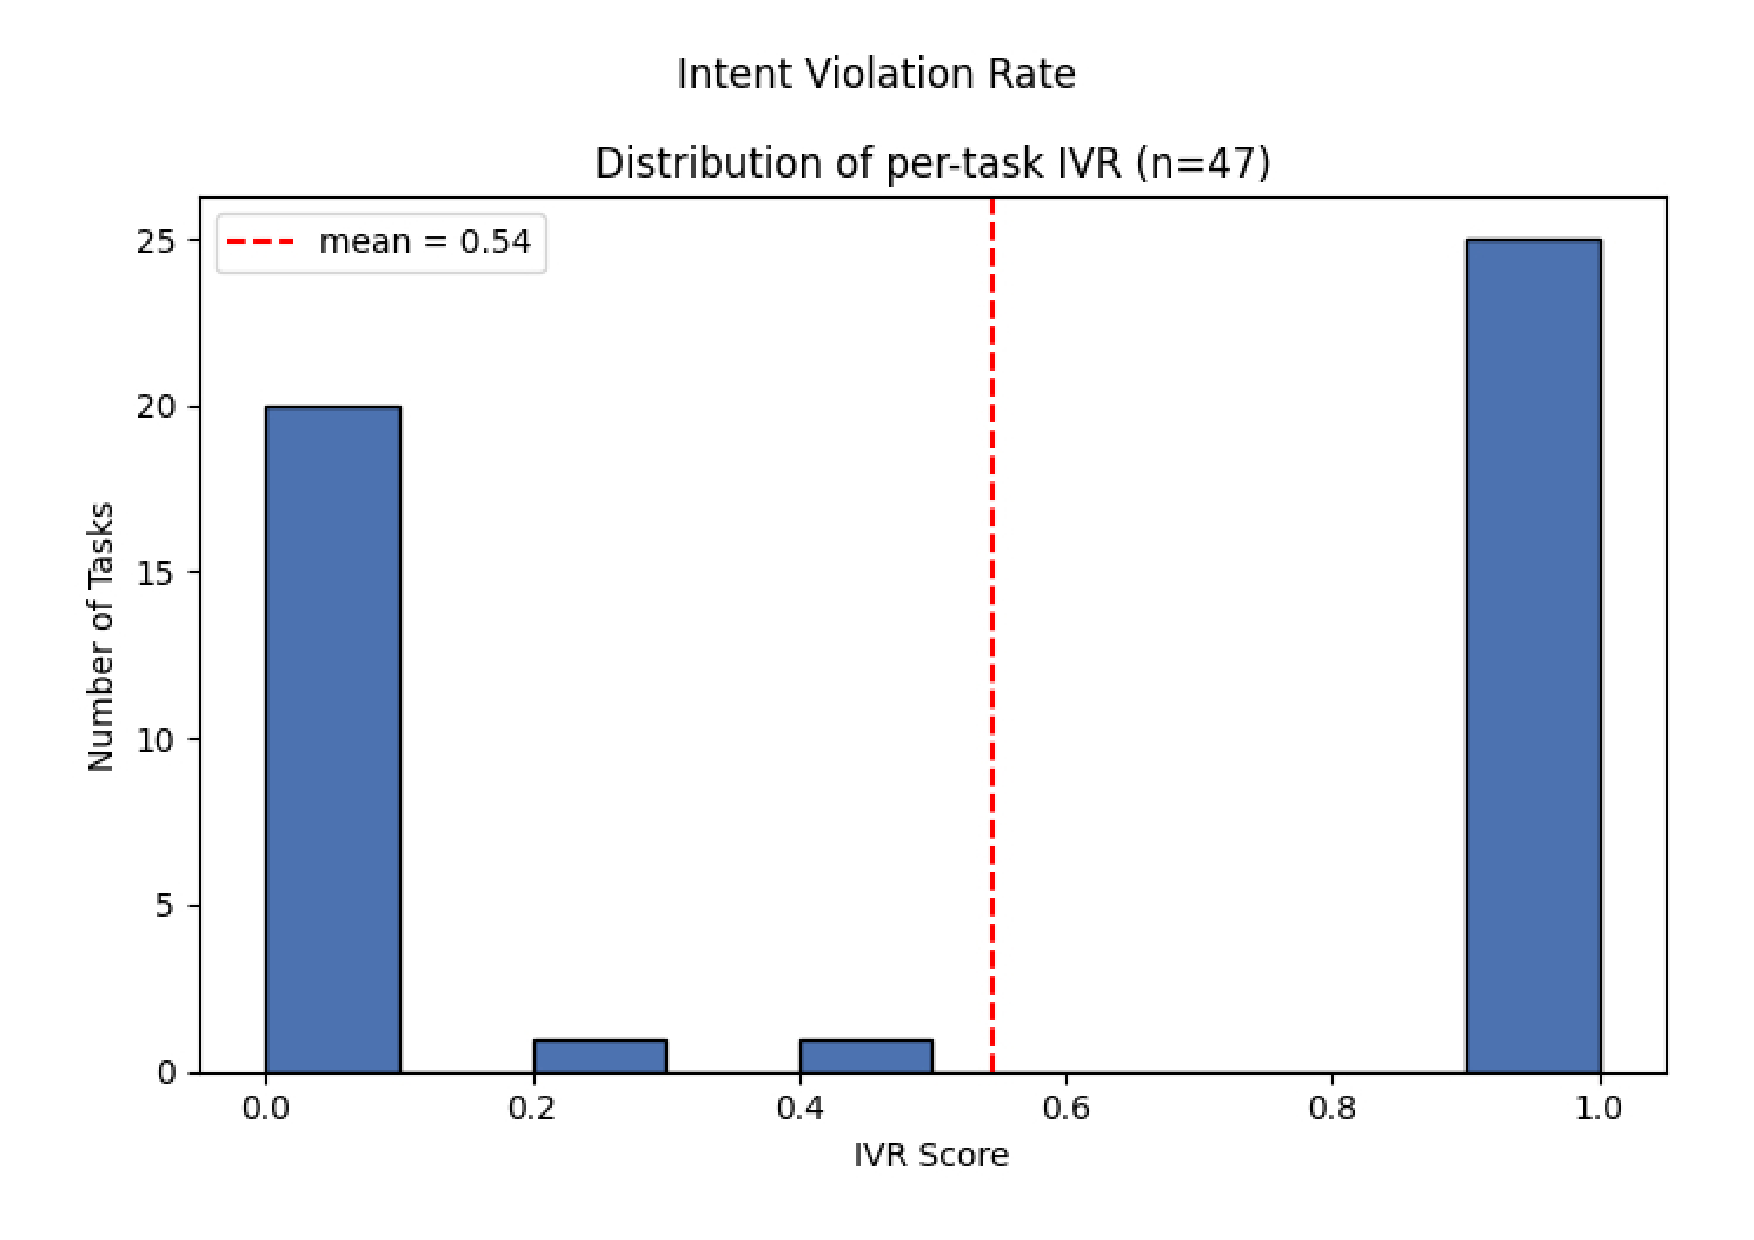
\includegraphics[width=\columnwidth]{ivr_distribution.pdf}
\caption{Distribution of per-problem IVR for Claude
Sonnet 4.6 across 47 spec pairs. Two problems with no stated-test-passing solutions are excluded.}
\label{fig:distribution}
\end{figure}

Figure~\ref{fig:distribution} shows a breakdown of the problems that pass the stated test and their level of violation. 45 of the 47 problems that pass C1 are at the extremes.  
% \begin{table}[ht]
% \centering
% \begin{tabular}{@{}lc@{}}
% \toprule
% \textbf{Per-problem IVR} & \textbf{\# Problems} \\
% \midrule
% $\mathrm{IVR} = 0.0$ (never violated)   & 20 \\
% $0 < \mathrm{IVR} < 1.0$ (mixed)        & 2 \\
% $\mathrm{IVR} = 1.0$ (always violated)  & 25 \\
% \midrule
% Total (with $\geq 1$ C1-pass)           & 47 \\
% \bottomrule
% \end{tabular}
% \caption{Distribution of per-problem IVR for Claude
% Sonnet 4.6 across 47 spec pairs. Two problems with no stated-test-passing solutions are
% excluded.}
% \label{tab:distribution}
% \end{table}

The mean IVR of 54.5\% reflects the bimodal split we see, with problems tending to cluster at IVR = 0 (no solutions violate intent) or IVR = 1 (every solution violates intent), with 45 out of 47 at these extremes. This near-deterministic behavior indicates that intent violations are systematic properties of a given task rather than sampling noise. If violations came from random variation in generation, per-problem IVR would be spread across intermediate values. Instead, the model consistently produces outputs that either fail to capture hidden constraints or fully do so.

The stated test C1, fails significantly less than hidden tests, at 5.7\%. Compared to hidden test fail rates, C1 is roughly 37 points lower than C2 (42.9\%), and is about 10 points lower the least-violated hidden constraint, C4 (15.4\%). 

\begin{table}[ht]
\centering
\begin{tabular}{@{}lccc@{}}
\toprule
\textbf{Constraint} & \textbf{Present} & \textbf{Failed} & \textbf{Fail Rate} \\
\midrule
C1 (stated)   & 245 & 14 & 5.7\% \\
C2 (hidden)   & 231 & 99 & 42.9\% \\
C3 (hidden)   & 201 & 58 & 28.9\% \\
C4 (hidden)   & 65  & 10 & 15.4\% \\
\bottomrule
\end{tabular}
\caption{Failure rate by constraint for Claude Sonnet 4.6
across 49 algorithm spec pairs (245 solutions). The stated
test (C1) is rarely failed, but hidden intent constraints
fail far more often. ``Present'' counts solutions whose problem
included the constraint; C2--C4 rates are over
stated-test-passing solutions.}
\label{tab:main-results}
\end{table}

\subsection{Analysis}
Hidden constraints are numbered in the order they were decomposed from the gold prompt, and this ordering is positional and does not strictly rank constraints by centrality. We nonetheless observe that earlier numbered constraints fail more often than later ones (Table~\ref{tab:main-results}), which may indicate that the first stripped constraint is often most central to the task, while later constraints often capture narrower edge cases. 

If we refer to HumanEval 34 in Section 3.2, it has a calculated IVR of 1.0, with all 5 solutions passing the stated test C1: return unique values, but those same solutions all failed the hidden constraint C2: sorted ascending order. However, in HumanEval 25, the ambiguous prompt reads as "Write a function named solution that returns the prime factors of a given integer", and this problem also contains the hidden constraint of returning the output in ascending order, and across all 5 solutions, it passes this constraint and others, reporting a IVR of 0.0. This suggests that intent satisfaction is constraint-dependent and context-dependent, rather than uniform. 

% ============================================================
% 5. CONCLUSION 
% ============================================================
\section{Conclusion}

We introduced the Intent Violation Rate (IVR), a metric that measures how often LLM generated code passes its stated tests, while violating unstated developer intent, and a small pilot benchmark of N=49 audited algorithm specification pairs derived from HumanEval+. Evaluating Claude Sonnet 4.6 on this benchmark, we found that despite 94.3\% of solutions passing stated tests, the model produced code that violated at least one hidden intent constraint in 54.5\% of problems. These violations fell into a systematic and near-deterministic pattern, rather than random noise, indicating that functional correctness metrics can overstate how well generated code reflects what a developer actually intended. Future work includes detecting underspecification before generation, expanding the benchmark, and extending IVR across additional models and task domains. 

% ============================================================
% LIMITATIONS — REQUIRED. Unnumbered, after conclusion,
% before references. Does NOT count toward the 4 pages.
% Discussion only: no new experiments, figures, or analysis.
% ============================================================
\section*{Limitations}

Our experiment and benchmarking was only tested on the Claude Sonnet 4.6 model, at a single temperature of 1.0. IVR could differ across models and lower temperatures. Additionally, the benchmark is small, with only N=49, limiting statistical power, with constraint type distributions being more suggestive, than robust. The benchmark also only focuses on Python algorithmic problems only, other languages and other problem types such as data transformation may have different findings. The problem specification is constrained to single-annotation construction, therefore the defined behavior of clarified gold prompts and tests reflect the judgment of one person. This also affects the operationalized definition of "intent", as we do not measure "intent" in an absolute metric. Also, HumanEval+ is a public dataset, it is possible that the model has seen the original problems in training prior to our experimentation. 

% ============================================================
% ETHICAL CONSIDERATIONS — optional, free space.
% ============================================================
\section*{Ethical Considerations}
\todo{E.g.: implications of deploying LLM-generated code that silently violates intent; benchmark contamination considerations; licensing of source datasets.}

% ============================================================
% ACKNOWLEDGMENTS — camera-ready ONLY. Leave commented out
% for the anonymous submission.
% ============================================================
% \section*{Acknowledgments}
% TODO after acceptance

% ============================================================
% REFERENCES — unlimited pages
% Include DOIs/URLs in every entry where possible.
% ============================================================
\bibliography{custom,anthology-1,anthology-2}

% ============================================================
% APPENDICES — after references, letter-numbered, free space,
% double-column format (default; don't switch to onecolumn
% unless a section is math-heavy). Must be supplemental only:
% the paper must stand alone without them.
% ============================================================
\appendix

\section{Spec Pair Construction Details}
\label{app:construction}
Construction Protocol: 
- Start from a HumanEval+ problem and its original prompt 
- Identify the implicit constraints the original problem specifies (ordering, edge-case handling, conditional behavior, etc.)
- Write a gold (clarified) prompt built off the original prompt that states all constraints explicitly; in some cases add specifics beyond the original to remove residual ambiguity 
- Strip the constraints from the gold prompt to produce the ambiguous prompt; omitting information that does not steer toward a wrong interpretation 
- Encode each stripped constraint as a hidden test (C2--C4); C1 is a stated test that must be satisfiable from the ambiguous prompt alone 
- Problems are algorithm only as they cleanly decompose into executable tests; other task types involve fuzzier constraints and lack a comparably licensed source at scale

\begin{table}[ht]
\small
\centering
\begin{tabular}{@{}p{0.9cm}p{6cm}@{}}
\toprule
\multicolumn{2}{@{}l}{\textbf{HumanEval/88} (conditional sort, IVR $=1.0$)} \\
\midrule
Ambig. & Return a sorted copy of a list of non-negative
         integers, without modifying the original. \\
\addlinespace
Gold & Sort ascending if the sum of the first and last
       elements is odd, descending if even; do not mutate
       the input. \\
\midrule
\textbf{C1} & \emph{stated}: sorts (odd sum) \newline
  \texttt{solution([2,4,3,0,1,5])} \newline
  \texttt{== [0,1,2,3,4,5]} \\
\addlinespace
\textbf{C2} & \emph{hidden}: descending on even sum \newline
  \texttt{solution([2,4,3,0,1,5,6])} \newline
  \texttt{== [6,5,4,3,2,1,0]} \\
\bottomrule
\end{tabular}
\caption{HE/88: the model sorts but ignores the
parity-dependent direction. All 5 solutions violate C2.}
\label{tab:ex-88}
\end{table}

\begin{table}[ht]
\small
\centering
\begin{tabular}{@{}p{0.9cm}p{6cm}@{}}
\toprule
\multicolumn{2}{@{}l}{\textbf{HumanEval/161} (fallback, IVR $=1.0$)} \\
\midrule
Ambig. & Swap the case of each letter, leaving non-letter
         characters unchanged. \\
\addlinespace
Gold & Swap the case of each letter; if the string
       contains no letters, return it reversed instead. \\
\midrule
\textbf{C1} & \emph{stated}: case swap \newline
  \texttt{solution('\#a@C') == '\#A@c'} \\
\addlinespace
\textbf{C2} & \emph{hidden}: reverse if no letters \newline
  \texttt{solution('1234') == '4321'} \\
\bottomrule
\end{tabular}
\caption{HE/161: the model performs the case swap but
misses the no-letters fallback. All 5 solutions violate C2.}
\label{tab:ex-161}
\end{table}

\begin{table}[ht]
\small
\centering
\begin{tabular}{@{}p{0.9cm}p{6cm}@{}}
\toprule
\multicolumn{2}{@{}l}{\textbf{HumanEval/25} (satisfied, IVR $=0.0$)} \\
\midrule
Ambig. & Return the prime factors of a given integer. \\
\addlinespace
Gold & Return the prime factors in ascending order, with
       repeated factors and product equal to the input. \\
\midrule
\textbf{C1} & \emph{stated}: basic factorization \newline
  \texttt{solution(13) == [13]} \\
\addlinespace
\textbf{C2} & \emph{hidden}: ascending order \newline
  \texttt{solution(15) == [3,5]} \\
\bottomrule
\end{tabular}
\caption{HE/25: the ascending-order constraint is
satisfied by all 5 solutions, as standard factorization
emits factors in ascending order. Contrast with HE/34,
where the analogous ordering constraint is violated.}
\label{tab:ex-25}
\end{table}

\subsection*{Validation Detail}
The benchmark was validated in two passes.

\textbf{Leakage audit.} Each stated test (C1) must be
satisfiable from the ambiguous prompt alone, without
knowledge of any hidden constraint. Of the 49 problems,
9 initially failed this check: type errors, output-format
contamination (e.g., a list expected where a tuple was
returned), and hidden-constraint leakage, where C1
inadvertently tested a hidden constraint so that no
solution could pass C1 without already encoding part of
the intent. All 9 were corrected.

\textbf{Canonical soundness check.} We ran the HumanEval+
canonical solution for each problem against the full test
suite (C1 and all hidden constraints); a correct solution
must pass all constraints, yielding IVR $=0$. This surfaced
2 further problems whose tests were themselves faulty
rather than leaked: HE/47 had an incorrect expected median
value, and HE/18 contained a contradictory empty-substring
constraint. Both were corrected (the HE/18 constraint was
removed, as the empty-substring convention is ambiguous).
After correction, all 49 canonical references yield
IVR $=0$, confirming the hidden tests are satisfiable by
correct code.

\section{Prompts and Sandbox Configuration}
\label{app:prompts}
Write a Python function named `solution` that solves the following task.
{prompt}
Requirements:
- Name the function exactly `solution`.
- Return only the function definition — no explanation, no markdown,
  no imports unless the function itself needs them.

Where {prompt} is the ambiguous prompt. 

Decoding Parameters: 
- Model: Claude Sonnet 4.6 
- Temperature: 1.0 (API default)
- Max Tokens: 1024 
- Number Samples per Problem: 5 

Post Processing: Markdown code fences are stripped from model output before execution to prevent ... 

Sandbox: Subprocess-based execution, one subprocess per test, 5-second timeout per test, adapted from HumanEval's execution harness (process isolation, syscall restrictions). Each solution is run against C1 (stated test) and each hidden constraint independently. 

\section{Per-Problem Results}
\label{app:results}
Table~\ref{tab:per-problem} reports the per-problem IVR for all 49 spec pairs,
the number of solutions passing the stated test (C1) out of 5, and which hidden
constraints were violated. HE/101 and HE/112 had no C1-passing solutions and are
excluded from the IVR mean.

\begin{table}[ht]
\centering
\small
\begin{tabular}{@{}lccl@{}}
\toprule
\textbf{Problem} & \textbf{C1 pass} & \textbf{IVR} & \textbf{Violated} \\
\midrule
HE/7 & 5/5 & 0.00 & -- \\
HE/12 & 5/5 & 0.40 & C3 \\
HE/18 & 5/5 & 0.00 & -- \\
HE/20 & 5/5 & 0.00 & -- \\
HE/21 & 5/5 & 0.00 & -- \\
HE/25 & 5/5 & 0.00 & -- \\
HE/26 & 5/5 & 0.00 & -- \\
HE/30 & 5/5 & 0.00 & -- \\
HE/34 & 5/5 & 1.00 & C2 \\
HE/42 & 5/5 & 0.00 & -- \\
HE/47 & 5/5 & 0.00 & -- \\
HE/51 & 5/5 & 0.00 & -- \\
HE/57 & 5/5 & 1.00 & C2 \\
HE/58 & 5/5 & 1.00 & C2,C3 \\
HE/64 & 5/5 & 1.00 & C2,C3 \\
HE/65 & 5/5 & 1.00 & C3 \\
HE/66 & 5/5 & 1.00 & C2 \\
HE/68 & 5/5 & 0.00 & -- \\
HE/70 & 5/5 & 0.00 & -- \\
HE/71 & 5/5 & 1.00 & C2,C3 \\
HE/72 & 5/5 & 1.00 & C2 \\
HE/74 & 5/5 & 0.00 & -- \\
HE/86 & 5/5 & 1.00 & C2,C3 \\
HE/88 & 5/5 & 1.00 & C2 \\
HE/90 & 5/5 & 1.00 & C3,C4 \\
HE/91 & 5/5 & 1.00 & C2,C3 \\
HE/93 & 5/5 & 1.00 & C2,C3 \\
HE/95 & 5/5 & 1.00 & C4 \\
HE/98 & 5/5 & 0.00 & -- \\
HE/99 & 5/5 & 0.00 & -- \\
HE/101 & 0/5 & -- & -- \\
HE/102 & 5/5 & 1.00 & C3 \\
HE/104 & 5/5 & 1.00 & C2 \\
HE/105 & 5/5 & 0.20 & C2 \\
HE/108 & 1/5 & 0.00 & -- \\
HE/111 & 5/5 & 1.00 & C2,C3 \\
HE/112 & 0/5 & -- & -- \\
HE/120 & 5/5 & 0.00 & -- \\
HE/126 & 5/5 & 1.00 & C3 \\
HE/131 & 5/5 & 0.00 & -- \\
HE/135 & 5/5 & 0.00 & -- \\
HE/136 & 5/5 & 0.00 & -- \\
HE/140 & 5/5 & 1.00 & C2 \\
HE/145 & 5/5 & 1.00 & C2 \\
HE/149 & 5/5 & 1.00 & C2 \\
HE/151 & 5/5 & 1.00 & C2 \\
HE/158 & 5/5 & 1.00 & C2 \\
HE/161 & 5/5 & 1.00 & C2 \\
HE/163 & 5/5 & 1.00 & C2,C3 \\
\bottomrule
\end{tabular}
\caption{Per-problem IVR across all 49 spec pairs. ``C1 pass'' is the
number of the 5 sampled solutions passing the stated test; ``IVR'' is the
fraction of those that violate $\geq 1$ hidden constraint; ``Violated''
lists the hidden constraints failed by any C1-passing solution.}
\label{tab:per-problem}
\end{table}
\end{document}